\documentclass[12pt]{report}
\usepackage[utf8]{inputenc}
\usepackage{graphicx}
\usepackage{listings}
\usepackage{float}
\usepackage{amsmath,amsfonts,amssymb}
\usepackage{geometry}
\geometry{a4paper,textheight=650pt,textwidth=400pt}

\title
{
{Modeling Resource Allocation Strategies in Annual Social Insects}\\
{\large MATH 463: Biomathematics}\\
{\large Dr. Jason Graham} \\
{
\includegraphics{university.png}}
}
\author{Maxwell Greene}
\date{\today}

\usepackage{Sweave}
\begin{document}
\Sconcordance{concordance:SweaveDoc.tex:SweaveDoc.Rnw:%
1 19 1 1 0 2 1 1 13 65 1 1 22 23 1 1 30 41 1 4 0 1 3 17 1 1 34 1 2 9 1 %
1 29 9 1 1 39 1 2 16 1 1 28 9 1 1 38 1 2 11 1}



\maketitle

\tableofcontents
\listoffigures
\addcontentsline{toc}{chapter}{Abstract}

\chapter*{Abstract}

The classic model of queen resource allocation by Macevicz and Oster predicts maximal fitness with a “bang-bang” strategy; an initial investment phase of worker rearing, followed by a production phase of solely reproductive rearing. This has been well-verified with altered conditions and assumptions for continuous differential equation models. In the current study, these basic claims are investigated and the model to address a variety of conditions. I will show the simplicity and flexibility of this model, with slight variations to account for individual environmental conditions and colony strategies. In addition to observing the resulting dynamics of these equations, I will utilize the methods learned in MATH 463 to determine model characteristics such as steady states, as well as how these characteristics change under differing assumptions.


\addcontentsline{toc}{chapter}{Introduction}
\chapter*{Introduction}

The optimization problem of resource allocation has been well-studied in the context of numerous real-world scenarios such as economics \cite{harberger1995monopoly} and digital communication \cite{hui1988resource}. Similarly, organisms with reproductive and working capability must face a challenging problem: how must one balance investment and growth to achieve optimal fitness? As a result of social and eusocial insect colony structure (foraging workers and non-foraging reproductives), queens must formulate an answer to this problem. 

Annual social queens undergo distinct seasonal behavior due to weather changes, mainly temperature fluctuation. Namely, queens and their offspring must "overwinter, or bury underground" to survive harsh winter months in some climates. This overwintering results in necessitated death of all workers in annual colonies, meaning only queens will survive the next season, restarting the annual cycle once they emerge. The resulting queens will start new colonies, each carrying the genetic material of their mother queens, thus giving the mother higher fitness for each reproductive that survives their overwinter.

Macevicz and Oster incorporated this idea to address reproductive strategies of annual eusocial colonies \cite{macevicz1976modeling}. They proposed what they termed the “bang-bang” strategy; an initial investment phase of worker rearing, followed by a production phase of reproductive rearing. Several theoretical models \cite{mitesser2007optimal,mitesser2007adaptive} and empirical studies \cite{greene1984production,ode2002resource} have followed, each modifying assumptions or model parameters for a given species including multiple vespine wasp species \cite{greene1984production} and the harvester ants \textit{Messor pergandei} \cite{ode2002resource}. Empirical strategies other than “bang-bang” are often interpreted as a bet-hedging response, creating a more robust strategy against environmental conditions. In fact, Mitesser et al. \cite{mitesser2007adaptive} showed a critical level of environmental variation for which bet-hedging became optimal. Therefore, bet-hedging may not be the reason for graded control, at least in conditions with relatively low environmental variation. 

While these empirical studies are insightful for the dynamics of a single species, the associated model parameters vary greatly between species and environment. Thus, it would provide great utility to generalize this model to account for the behaviors of the majority of species facing the same dilemma. 


\chapter*{Results}
\addcontentsline{toc}{chapter}{Results}
While queens often reproduce over multiple colony cycles, many species experience a distinct cycle in which a queen loses all reproductives and workers. Thus, I accompany the majority of the literature in quantifying queen fitness as the number of reproductives alive at the end of a colony cycle. Here I presume that queens employ some strategy to optimize reproductive numbers and that they may possess biological mechanisms to inform and make this series of investment/growth choices. For the purpose of simplicity I define this function with respect to time. In the continuous case, reproductive strategy is defined as the percent of resource allocated to reproductive rearing.

Forager death rate alone has been shown to account for external environmental factors in colony population dynamics \cite{khoury2011quantitative}, making this a simple and effective way to model environmental effects. Thus, in the standard case I describe environment by the forager death rate throughout the season. I will then use additional parameters including resource availability to define further environmental effects. 

Since all colony members depend on the same energy type (honey) from the same source (foraging trips) I use it as a basis for all colony functions. A conversion factor for production and consumption of energy is representative of the time investment for foraging trips and rearing brood.

Eusocial insects have evolved to fill very specific ecological niches, yet there is large variation in the climates and environments in which they survive. For instance, while some species overwinter due to freezing conditions, others are able to continue throughout the cold season. Heinrich and Bernd \cite{heinrich1976resource} have quantified the number of flowering species and temperatures for a number of climates, which suggests that unimodal functions may not be representative of the environment. Therefore, to account for all possible environments and associated strategies, it is likely that one would have to consider a variety of functions. For the sake of simplicity, the earlier models are limited to linear combinations of second degree polynomials modelling a 3-season reproductive cycle. However, I will proceed to investigate a variety of functions and the resulting colony dynamics.


%\section*{Classical Model}
%\addcontentsline{toc}{section}{Classical Model}

\section*{Compartment Diagram}
\addcontentsline{toc}{section}{Compartment Diagram}
The system of equations in eq. (\ref{eq: system}) describes the compartment diagram in figure \ref{fig: Compartment Diagram}. Three main quantities are modelled: energy, worker population and reproductive population. Worker and reproductive population are each dependent on the energy quantity, but reproductives only contribute under certain circumstances. Workers contribute to energy at a rate of $Kw$, energy per worker per time. For the purpose of simplicity, the $K_r$ value is held constant at $0$ for all systems with initial conditions $E=1, W=0, R=1$. Energy is allocated to the populations using the $Br$ quantity, which represents the fraction of reproductive resources being invested in reproductives. See table \ref{table: variables} for a summary of variables and parameters used. 

\begin{table}
\begin{tabular}{||c l l |}
\hline
 
%%%%%%%%%%%%%%%%%%%%%%%%%%%%%%
%%%%% Table of Variables %%%%%
%%%%%%%%%%%%%%%%%%%%%%%%%%%%%%

 Variable & Description (IV - Independent Variable, DV - Dependent Variable) & Units  \\ [0.5ex] 
 \hline\hline
 $R$  & DV: Number of Reproductives 			& $reproductives$ \\  [5pt]
 $W$ & DV: Number of Workers    					& $workers$ \\ [5pt]
 $E$  & DV: Amount of Energy 							& $energy$ \\  [5pt]
 $D_w$& IV: Worker Death Rate 							& $\frac{1}{time}$  \\   [5pt]
 $D_r$ & IV: Reproductive Death Rate 				& $\frac{1}{time}$   \\  [5pt]
 $B_r$ & IV: Birthing fraction for reproductives.  *Note $B_w = 1-B_r$  & $1$  \\  [5pt]
 $C_w$& IV: Conversion factor, energy required to create a worker. & $\frac{worker}{energy * time}$ \\  [5pt]
 $C_r$ & IV: Conversion factor, energy required to make a reproductive & $\frac{reproductve}{energy * time}$ \\ 
 $K_w$& IV: Conversion factor, energy foraging rate per worker & $\frac{energy}{worker * time}$ \\  [5pt]
 $K_r$ & IV: Conversion factor, energy foraging rate per reproductive & $\frac{energy}{reproductive * time}$ \\  [5pt] \hline
\end{tabular}
\label{table: variables}
\caption{Variables used in continuous model, figure \ref{fig: Compartment Diagram}.}
\end{table}

\begin{figure}
	\centering
    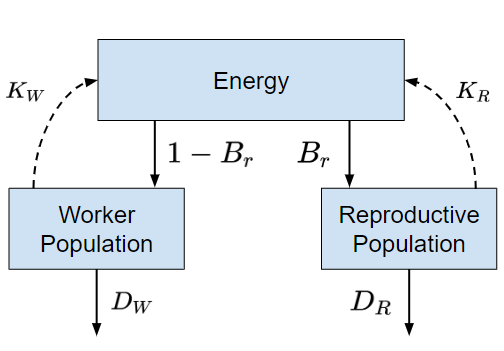
\includegraphics[width=0.65\textwidth]{compartmentdiagram.png}
    \caption{Compartment diagram described by the system of equations in \ref{eq: system}.  See variable summary in \ref{table: variables}. Energy accounting for all colony actions, meaning any population or colony function is described by its interaction with the energy quantity. }
    \label{fig: Compartment Diagram}
\end{figure}

%%%%%%%%%%%%%%%%%%%%%%%%%%%%%%%%%%
%%% Compartment Diagram System %%%
%%%%%%%%%%%%%%%%%%%%%%%%%%%%%%%%%%

\section*{Analysis of Differential Equation System}
\addcontentsline{toc}{section}{Analysis of Differential Equation System}

\begin{equation}
\begin{aligned}
\frac{dW}{dt}&=\frac{1-B}{C_w}E-D_w W\\
\frac{dR}{dt}&=\frac{B}{C_r}E-D_r R\\
\frac{dE}{dt}&=K_w W + K_r R - E
\end{aligned}
\label{eq: system}
\end{equation}



%%%%%%%%%%%%%%%%%%%%%%%%%%%%%%%%%%
%%%%% Non-Dimensionalization %%%%%
%%%%%%%%%%%%%%%%%%%%%%%%%%%%%%%%%%

\subsection*{Non-Dimensionalization}
\addcontentsline{toc}{subsection}{Non-Dimensionalization}

Non-dimensionalization of this system gives the following:

\begin{equation}
\begin{aligned}
\frac{dW}{d\tau}&=w E-W \\
\frac{dR}{d\tau}&=r E-R \\
\frac{dE}{d\tau}&=  W+R
\end{aligned}
\label{eq: nondim}
\end{equation}

where

\begin{equation}
\begin{aligned}
&w=\frac{(1-B) k_w}{C_w D_w^2}\\
&r=\frac{B k_r}{C_r D_r^2}\\
\end{aligned}
\label{eq: nondim wr}
\end{equation}

with substitutions

\begin{equation}
\begin{aligned}
W &= \frac{D_w E_{c}}{K_w}W_1
&&R = \frac{D_r E_{c}}{K_r}R_1\\
E &= E_c E_1  &&t = \frac{1}{D_w}\tau
\end{aligned}
\label{eq: subs}
\end{equation}

\begin{Schunk}
\begin{Sinput}
> #Include non-dimensionalization definition
\end{Sinput}
\end{Schunk}

Where $E_c$  is a critical energy level, which can represent a number of biological quantities. Others have discussed issues such as resource limitation on the queen \cite{mitesser2007optimal} or environmental factors such as energy availability or nest size. This particular scaling would certainly aid in modelling energy-limiting factors. Finally, $\frac{1}{Dw}$ scales time well under constant death rate conditions, but is nonlinear under realistic, variable death rate environmental conditions.

\subsection*{Steady States}
\addcontentsline{toc}{subsection}{Steady States}

\section*{Standard System Dynamics}
\addcontentsline{toc}{section}{Standard System Dynamics}

%\begin{figure}[t]
%\centering
%    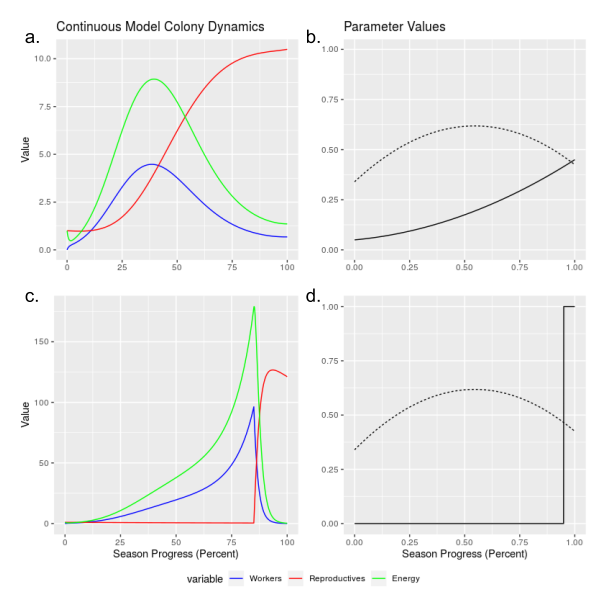
\includegraphics[width=0.75\textwidth]{continuousall.png}
%    \caption{Colony dynamics for the system of equations (a,c) with corresponding parameters on the right side graphs (b,d). Dashed lines represent forager death rate, while solid black line represents percent allocation of resources to reproductive rearing. Forager death rate used here is a monotonic linear combination of second degree polynomial functions. The parameters in (a,b) represent a bet-hedging approach and those in (c,d) represent the "bang-bang" strategy with transition point such that all energy can be converted to reproductives.}
%    \label{fig: Continuous dynamics}
%\end{figure}

\begin{figure}[t]
\centering
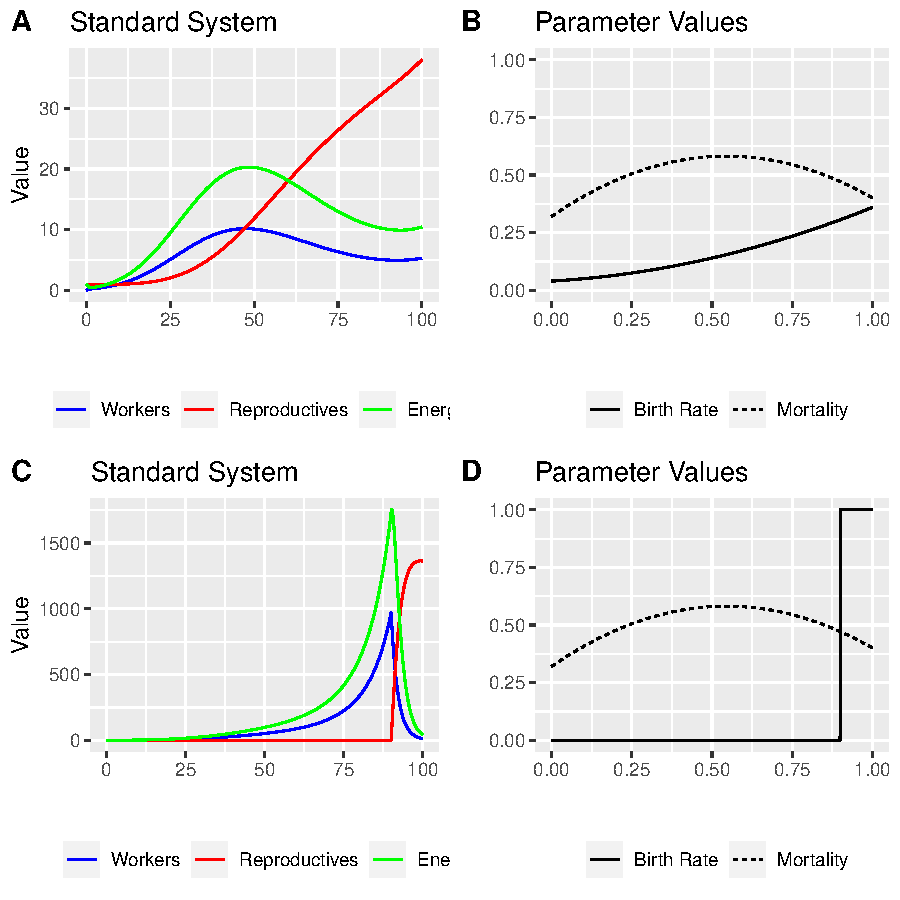
\includegraphics{SweaveDoc-005}
\caption{Colony dynamics for the system of equations (a,c) with corresponding parameters on the right side graphs (b,d). Dashed lines represent forager death rate, while solid black line represents percent allocation of resources to reproductive rearing. Forager death rate used here is a monotonic linear combination of second degree polynomial functions. The parameters in (a,b) represent a bet-hedging approach and those in (c,d) represent the "bang-bang" strategy with transition point such that all energy can be converted to reproductives.}
\label{fig: Continuous dynamics}
\end{figure}
 
Regardless of the functions used to describe the system, one truth holds across parameter combinations: late season reproductive investment produces greater fitness. Figure \ref{fig: Continuous dynamics} (c)  illustrates the equivalent of the "bang-bang" strategy with the investment transition occurring just before the end of season, allowing conversion of all energy into reproductives. While others have discussed an optimal switching point or amount of bet-hedging \cite{poitrineau2009workers}, I am only concerned with verifying the existence of a fitness maximum. 

\section*{Resource Availability, Forager Success}
\addcontentsline{toc}{section}{Resource Availability, Forager Success}
While it is beyond the scope of the current study to investigate the precise effects of changing resource availability since it is independent of reproductive allocation, I would like to point to its great effect on colony success or failure. Figure \ref{fig: Continuous dynamics 2} illustrates the magnitude of these effects on reproductive output. The parameters for figures \ref{fig: Continuous dynamics} and \ref{fig: Continuous dynamics 2} are identical, apart from the changed resource availability (energy foraged per worker per day). This quantity is plotted (b,d) to illustrate the effects. Notably, the worker population is not able to support even itself given the decreasing resource availability and thus wastes energy attempting to maintain its population before investing in reproductives. Therefore, the "bang-bang" strategy may not be the most effective given a decreasing resource availability. A critical point is reached after which workers no longer forage as much energy as it took to rear them, having an overall negative effect. In all other cases, I hold resource availability constant at the arbitrary value 2. Another important consideration is that resource availability determines the extremes of a season and thus may act as scale of time in our continuous model. 


%\begin{figure}[t!]
%\centering
%    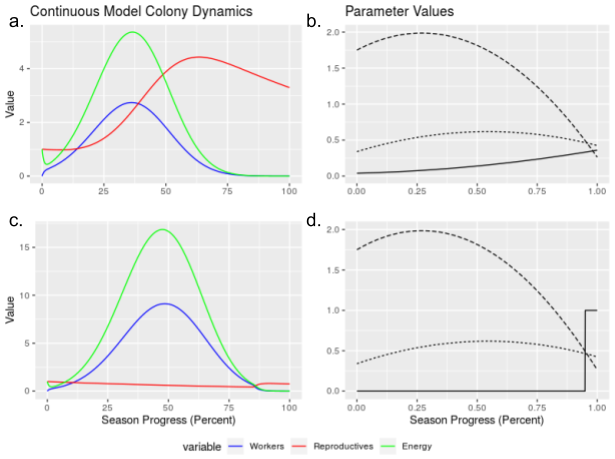
\includegraphics[width=\textwidth]{continuousall2.png}
%    \caption{Illustration of the effects of a changing resource availability on within-season colony dynamics. These systems consist of the same strategies and forager death rates used in figure \ref{fig: Continuous dynamics}, the only difference being resource availability. Long-dashed lines are resource availability (energy per forager per day) with the systems in figure \ref{fig: Continuous dynamics} using a constant 2 energy per forager per day. Short-dashed lines represent forager death rate, solid black line represents percent allocation of resources to reproductive rearing. Forager death rate used here is monotonic, a combination of polynomial functions.}
%    \label{fig: Continuous dynamics 2}
%\end{figure}

\begin{figure}[t!]
\centering
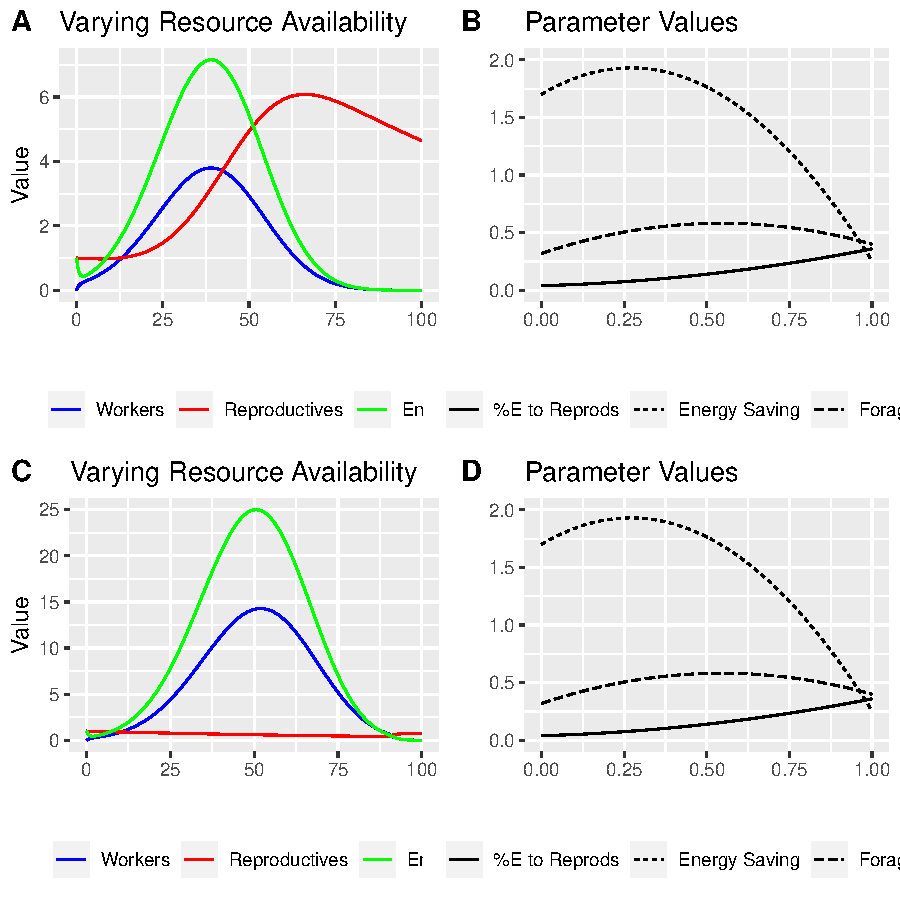
\includegraphics{SweaveDoc-007}
\caption{Illustration of the effects of a changing resource availability on within-season colony dynamics. These systems consist of the same strategies and forager death rates used in figure \ref{fig: Continuous dynamics}, the only difference being resource availability. Long-dashed lines are resource availability (energy per forager per day) with the systems in figure \ref{fig: Continuous dynamics} using a constant 2 energy per forager per day. Short-dashed lines represent forager death rate, solid black line represents percent allocation of resources to reproductive rearing. Forager death rate used here is monotonic, a combination of polynomial functions.}
\label{fig: Continuous dynamics 2}
\end{figure}

\section*{Energy Provisioning}
\addcontentsline{toc}{section}{Energy Provisioning}
Most models in the literature make the assumption that all gathered energy is immediately converted into either a worker or a reproductive. However, natural colonies have a tendency to store energy without a complete conversion. (Apiarists exploit this behavior to overproduce and collect honey for human consumption.) This energy preservation is another form of bet-hedging, where the resource is stored as energy rather than as reproductives. Thus, a "preservation" parameter, $P_e$, can easily be added to the system to model this behavior. For example, if we have $P_e=0.25$ then 25\% of energy is stored, while 75\% is used for producing workers and reproductives. The system below exemplifies this modification.

\begin{equation}
\begin{aligned}
\frac{dW}{dt}&=\frac{(1-B)(1-P_e)}{C_w}E-D_w W\\
\frac{dR}{dt}&=\frac{B(1-P_e)}{C_r}E-D_r R\\
\frac{dE}{dt}&=K_w W + K_r R - (1-P_e)E
\end{aligned}
\label{eq: energy system}
\end{equation}


%\begin{figure}[t!]
%\centering
%    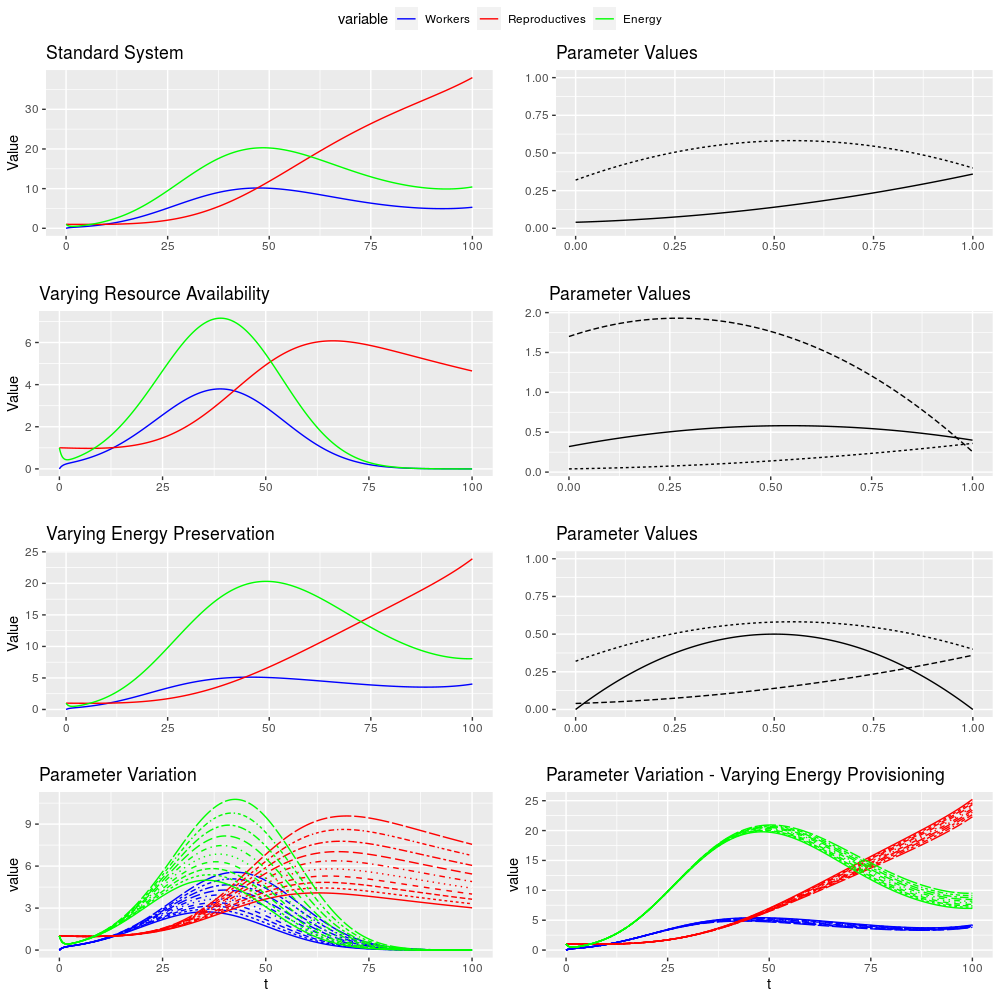
\includegraphics[width=\textwidth]{alldraft.png}
%    \caption{}
%    \label{fig: all plots draft 1}
%\end{figure}

\begin{figure}[t]
\centering
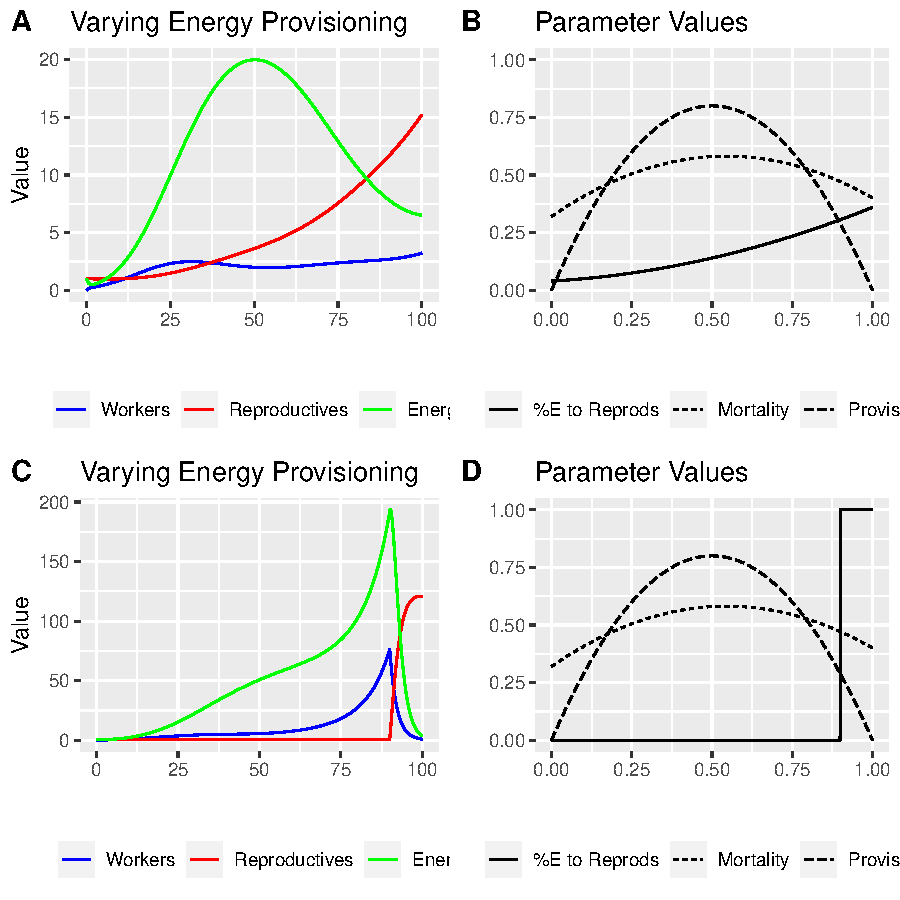
\includegraphics{SweaveDoc-temp}
\caption{Result of energy provisioning strategy alongside standard (A) and bang-bang (C) strategies as described by the equations in equation \ref{eq: system}. Associated parameters are illustrated on the right (B,D). The provisioning stratedy presented here is monotonic, with high provisioning in the early season. }
\end{figure}

%\chapter*{Conclusion}
%\addcontentsline{toc}{chapter}{Conclusion}

\newpage

\bibliographystyle{plain}
\bibliography{references.bib}

\end{document}
